%*****************************************
\chapter{3D Spieleentwicklung mit Java}\label{ch:beispiele}
%*****************************************

\section{Allgemeiner Aufbau von 3D Spielen}\label{sec:aufbau}

Bei 3-dimensionalen Spielen wird das Spielgeschehen in einen Raum transferiert und dem Spieler die Möglichkeit gegeben sich dort frei bewegen zu können. \newline
Im Gegensatz zu 2-dimensionalen Spielen sind hier deutlich mehr Berechnungen auf vektorieller Ebene notwendig, was sich auf die Laufzeit niederschlägt. Daher ist es besonders wichtig ein effizientes Programm zu generieren.
Diesbezüglich ist Java nicht die optimale Programmiersprache, da durch den Interpreter viel Zeit verloren geht. \newline
Dennoch können mit Java sehr schöne und funktionale Spiele erstellt werden.
\\
Im Allgemeinen kann man sagen, dass die meisten 3D Spiele folgende Elemente enthalten:
\begin{itemize}
	\item 3D-Modelle und eine räumliche Spielumgebung
	\item Eine sog. "Kamera", welche nur den relevanten Teil des Bildes abbildet
	\item Möglichkeiten der Interaktion
	\item Soundeffekte und Musik
\end{itemize}

\begin{figure}[h!]
		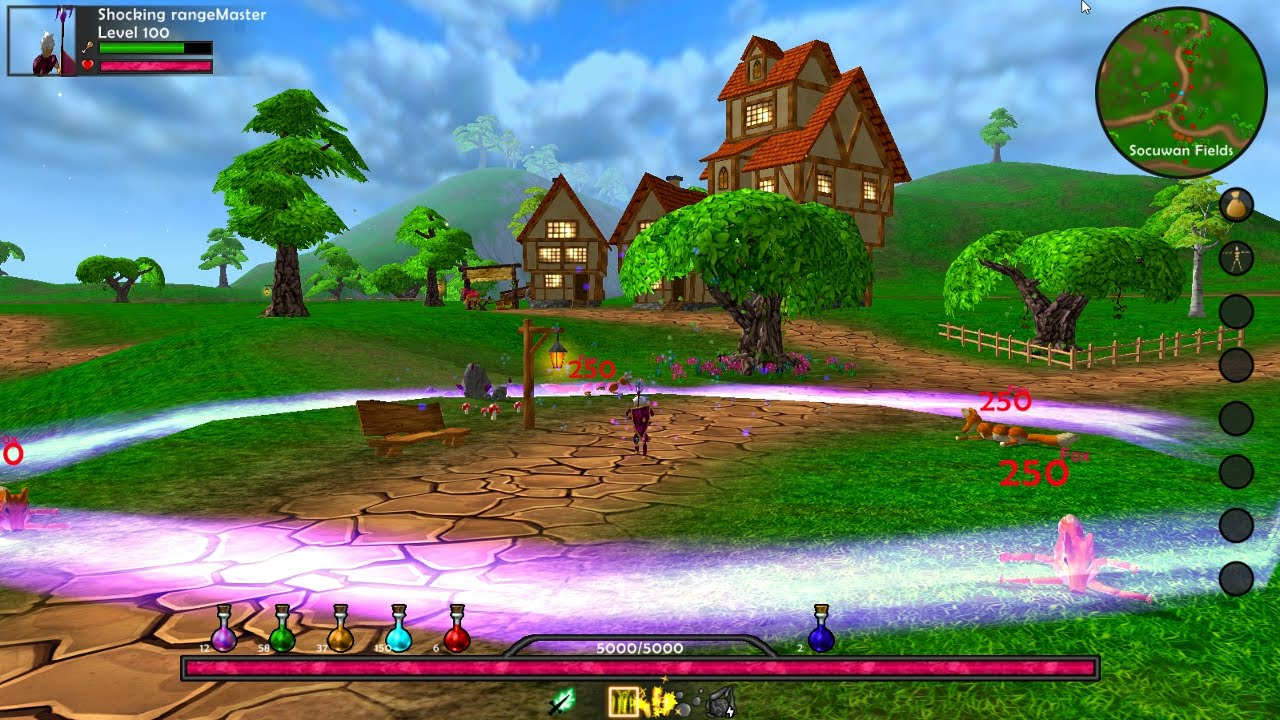
\includegraphics[width=1\linewidth, height = 200pt]{images/3dgame}
		\caption[Beispiel eines 3D Spiels]{Ausschnitt eines 3D Spiels in Java von ThinMatrix \cite{Fig2}}
	
\end{figure}

\clearpage

\section{Funktionsweise und Auswahl von Game Engines}\label{sec:jMonkeyEngine}
Um nicht sämtliche mathematischen Berechnungen auf der Grafikkarte selber programmieren, oder beispielsweise die Lautsprecher für Audio-Effekte ansprechen zu müssen, erhält der Entwickler Unterstützung durch sogenannte "Game Engines".
Diese beinhalten die Basisfunktionen von Spielen und ermöglichen dem Spiele-Programmierer eine gezieltere Entwicklung. Zu den Basisfunktionalitäten gehören im Allgemeinen die folgenden \cite{BF1}:
\begin{enumerate}
	\item Grafik-Engine
	\item Physiksystem
	\item Soundsystem
	\item Zustandsspeicherung
	\item Steuerung
	\item Datenverwaltung
\end{enumerate}
Zur Auswahl stehen eine Vielzahl von verschiedenen Engines, welche jeweils vor und Nachteile mit sich bringen. Da wir auf jeden Fall lernen wollten, wie die grundlegenden Dinge funktionieren, haben wir nach Engines gesucht, welche nur die Basisfunktionalitäten unterstützen, jedoch keine automatische Codegenerierung, Drag and Drop oder Editoren beinhalten.
Im folgenden eine Übersicht einiger Engines:


\begin{table}[h!]
	\myfloatalign
	\begin{tabularx}{\textwidth}{Xll} \toprule
		\tableheadline{GameEngine} & \tableheadline{Vorteile} & \tableheadline{Nachteile} \\ \midrule 
		Unity & Viele Benutzer, beliebt &  zu oberflächlich, kein Java \\
		jMonkeyEngine & Sehr entwicklungsnahe, Java & Schlechte Dokumentation \\
		Wurfel Engine & Benutzerfreundlich & Keine Physikunterstützung \\
		Cry Engine & Sehr schöne Grafik & Kein Java \\
		\bottomrule
	\end{tabularx}
	\caption[Engines]{Vor - und Nachteile einiger Game Engines \cite{GE1}}  \label{tab:example}
\end{table} 
Letztendlich fiel die Entscheidung auf die jMonkeyEngine, welche häufig von Java Entwicklern verwendet wird. 


\subsection {Die jMonkeyEngine}
Die jMonkeyEngine (jME) ist komplett in Java geschrieben und basiert auf dem Buch "3D Game Engine Design" von David Eberly \cite{GE2}.
Durch eine Abstraktionsschicht kann jedes beliebige Rendering System verwendet werden, beispielsweise die Lightweight Java Game Library (LWJGL) oder die Open Graphics Library (OpenGL).
Die neuste Version ist jME3, welche einige hilfreiche Funktionen mit sich bringt, wie beispielsweise ein Partikelsystem, Frustum Culling oder 3D Sound Unterstützung \cite{JM1}.
\begin{description}
	\item[Frustum Culling:] "Frustum Culling ist eine Optimierungsmethode, bei der all die Objekte vom Zeichnen ausgeschlossen werden, die außerhalb des Sichtbereichs (des Frustums) liegen." \cite{FC1}
\end{description}


\section{Umsetzung in Programmcode}\label{sec:code}
Im folgenden wird beschrieben wie einzelne Elemente in der jMonkeyEngine programmiert werden können und was dabei zu beachten ist. Die Erklärungen orientieren sich hierbei an dem jme3 Online-Beginners-Guide \cite{BG1} und der entsprechenden Dokumentation.

\subsection{Erzeugung der Application-Klasse: SimpleApplication}
Die Main-Klasse jedes jME3 Spieles erbt von der Klasse SimpleApplication, welche ein Spiel darstellt.
In der main-Methode wird dann eine neue Instanz erstellt und anschließend gestartet.

Jede Unterklasse der SimpleApplication beinhaltet die folgenden Methoden:
\begin{enumerate}
	\item simpleInitApp():
	Sorgt für das Laden von Modellen, der Erstellung einer räumlichen Umgebung sowie jegliche Initiierungen.
	\item simpleUpdate(float tpf):
	Wird für jedes frame per second (fps) ausgeführt und kümmert sich um gegebenenfalls geänderte Spielzustände.
	\item simpleRender(RenderManager rm):
	Wird stets nach simpleUpdate aufgerufen und zeichnet das Sichtbild des Spielers neu. Dazu bekommt die Methode einen RenderManager übergeben, welcher Präferenzen beim Zeichnen berücksichtigt (z.B. welche Ebene vorne oder hinten gezeichnet werden soll).
\end{enumerate} Die erste der drei Methoden wird stets zu Beginn ausgeführt um alle benötigten Elemente bereit zu stellen.

\subsection{Funktionsweise von Nodes}
Um Elemente zum Renderingprozess hinzuzufügen, um sie also sichtbar zu machen, müssen diese an ensprechende "Nodes" (engl. Knoten) angehängt werden.
Hierbei gibt es je nach Verwendungszweck verschiedene Arten zum Beispiel die \emph{audioNode} für Soundobjekte oder die \emph{guiNode} für Elemente auf der Benutzeroberfläche.\\
Final werden alle Nodes an die rootNode, also die Wurzel, angehängt. Im  Programmcode funktioniert dies mit der Methode \emph{attachChild()} bzw. \emph{detachChild()} zum entfernen.\\
Selbstverständlich können Objekte auch direkt an die rootNode angehängt werden, weshalb die Methodenparameter Modelle, Nodes, Bilder aber auch beispielsweise Audio-Files sind.
Allerdings ist es empfehlenswert eine geeignete Baumstruktur zu erstellen um so bestimmte Elemente in Gruppen anzusprechen.\\ \underline{\smash{Beispiel:}} Erzeugung einer eigenen Node durch:
\begin{lstlisting}
Node myNode = new Node();
myNode.doSomething();
\end{lstlisting}
Wird nun beispielsweise die folgende Funktion auf dem Konten ausgeführt, so wird diese auch für sämtliche Kinder des Knotens ausgeführt.





\subsection{Modelle und Assets}
Sämtliche externe Gegenstände des Spiels werden im \emph{assets}-Ordner im jME3 Projekt gesammelt. Dies sind multi-media Dateien wie 3D-Modelle, Soundfiles, Texturen, Shader und was sonst noch benötigt wird.
Um diese aus dem Ordner ins Spiel zu laden wird der sogenannte \emph{AssetManager} benötigt, welcher einfach eine Instanz der Klasse mit entsprechenden Funktionalitäten ist. \\Modelle sind dreidimensionale Gebilde welche verschiedenste Elemente in einem Spiel sein können. Hierbei verwendet jME3 die Klasse Spatial (engl. für "räumlich"). \\Zum Laden eines Objektes wird die entsprechende Funktion \emph{loadTexture(String path)} bzw. \emph{loadModel(String path)} aufgerufen und der entsprechende Pfad zum Modell übergeben:
\begin{center}
\fcolorbox{grau}{white}
{Spatial baum = assetManager.loadTexture("Models/Baum.j3o");}
\end{center} Für Modelle gibt es viele verschiedene Datentypen. Neben dem jMonkey-eigenen Dateiformat .j3o existieren einige weitere. Selbstverständlich ist meist eine Konversion zwischen den Formaten möglich. Die häufigsten von uns angetroffenen Vertreter für Modell-Deklarationen sind die folgenden:
\begin{enumerate}
	\item XML-Dateien: Aus einer mesh.xml Datei wird ein Objekt erzeugt. 
	\item OBJ-Dateien: Ein von \emph{Wavefront Technologies} entwickeltes Dateiformat für geometrische Formen. \cite{OBJ1}
	\item Blender-Dateien: Dies sind Dateien aus der Blender-Software, mit welcher Modelle erzeugt werden können.
\end{enumerate} Wie bereits unter \emph{Funktionsweise von Nodes} beschrieben müssen die Spatials nun lediglich zur rootNode, bzw. einer anderen Node welche mit der rootNode verknüpft ist, hinzugefügt werden. Damit werden die Modelle und Texturen sichtbar und sind Teil des Rendering-Prozesses.


\begin{center}
	\fcolorbox{grau}{white}
	{rootNode.attachChild(baum);}
\end{center} Der Aufbau von Modellen erfolgt durch entsprechende Software mit Polygonzügen oder Punktwolken. Dies definiert die allgemeine Struktur von Objekten.\\
Neben dieser und dem Material (vgl. \emph{Materialien}) gibt es noch das Skelett. Dieses kann ebenfalls in einem entsprechenden Programm wie Blender erzeugt und daraus bestimmte Bewegungsabläufe in Spielen bestimmt werden.
Das Skelett ist notwendig für Animationen von Modellen wie beispielsweise Gehen, Springen oder Ähnlichem.\\
In unserem Progman-Spiel haben wir uns für eine First-Person Perspektive entschieden, wodurch keine Animationen für den Spieler notwendig waren. Darüber hinaus haben wir uns auf Grund des Zeitaufwandes gegen eine Implementierung eines Skeletts beim Progman entschieden. Dieser ist daher nur eine starre Figur.



\subsection{Materialien}
Da in Modell-Software vorerst nur die Form von Figuren bestimmt wird, muss anschließend noch die Farbe, die Oberflächenstruktur und das Lichtverhalten bestimmt werden. Dies funktioniert über sogenannte \emph{'materials'}.\\
Die Datei für das Material kann in jme3 mit der Endung .mtl identifiziert werden. Diese bildet die entsprechenden Farbwerte von Bilddateien auf das Modell ab. Als Farbgeber sind beispielsweise mat.jpg oder mat.png gängig. Darüber hinaus können durch eine \emph{bump-map} und \emph{normalen}-Formate die Struktur der Oberfläche sowie das Verhalten bei Lichteinstrahlung (bspw. spiegelnd / schattierend /...) festgelegt werden. \\ Mit diesen Werkzeugen können sehr detaillierte Modellgenerierungen erfolgen, die nahezu realitätsgetreu sind.



\begin{figure}[h!]
	\myfloatalign
	\subfloat[Modell ohne Material]
	{
	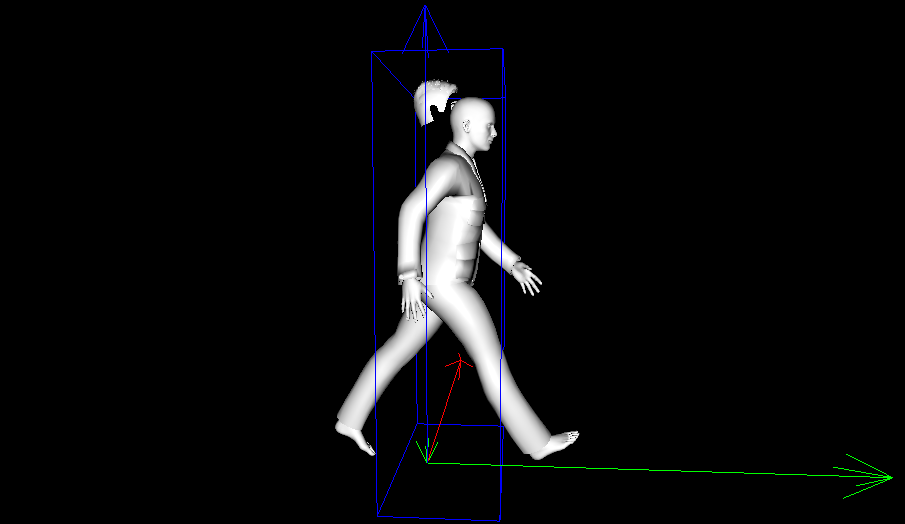
\includegraphics[width=.3\linewidth, height = 70pt]{images/modelmat}} \quad
	\subfloat[Modell mit Material]
	{\label{fig:example-b}%
	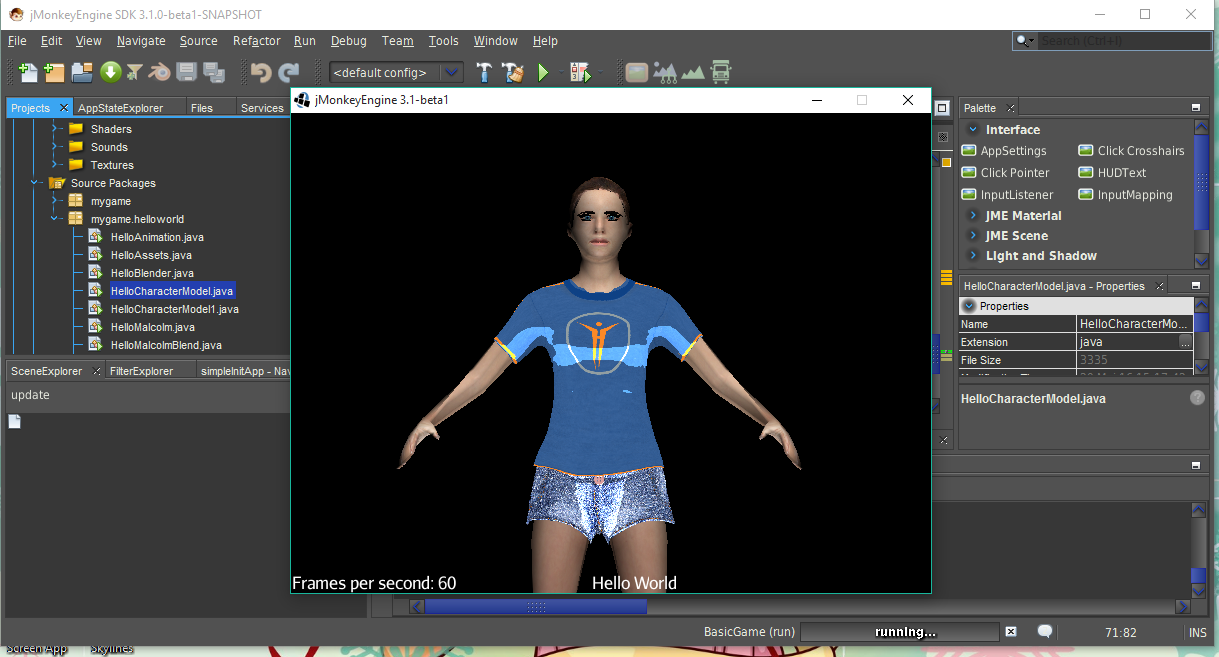
\includegraphics[width=.3\linewidth, height = 70pt]{images/modelmat2}} \\
	\caption[Materials auf Modellen]{Modell mit und ohne Material \cite{Fig1}}\label{fig:example}
	
\end{figure}







\subsection{User-Input}

Aus einem 3-dimensionalen Gebilde wird erst dann ein Spiel, wenn Interaktion mit dem Spieler stattfindet. Dazu müssen Tasteneingaben, Mauseingaben oder gegebenfalls auch Toucheingaben abgefangen und verarbeitet werden.
Hierbei werden die aus der ProkSy-Vorlesung bekannten Listener-Klassen verwendet.
Bezogen auf unser Spiel wurden folgende Aktionen durch Listener abgefangen:
\begin{enumerate}
	\item W/A/S/D: Dient zur Bewegung innerhalb des Spielraumes.
	\item Pfeiltasten/Maus: Zur Rundumsicht entsprechend einer Kopf-Bewegung.
	\item Taste "B": Aufnahme eines gefundenen Buches.
	\item Taste "L": Ein-/Ausschalten der Taschenlampe.
	\item Leertaste: Sprung
\end{enumerate} Zur Realisierung stehen in jme3 zwei wichtige Listener-Klassen zur Verfügung: Der \emph{ActionListener} und der \emph{AnalogListener}.
Ersterer sollte verwendet werden, wenn einzelne Aktionen erfolgen wie z.B. einmaliges Drücken der Taste B, zum Aufsammeln eines Buches.\\
Die zweite Klasse widerum, falls dauerhafte Events wie Gedrückthalten von W zur Vorwärtsbewegung abgefangen werden sollen. \\
Im Programmcode müssen dann entsprechende Aktionen erfolgen, damit der Input auch eine Auswirkung auf das Spiel hat. Beim Drücken von W müsste etwa der Richtungsvektor sowie die aktuelle Position abgefangen werden um eine Vorwärtsbewegung um x = walkingSpeed Richtungseinheiten zu erzeugen.

\subsection{Kollisionserkennung}
Damit man als Charakter nicht durch die gesamte Spielwelt gehen kann, müssen entsprechende Kollisionserkennungen eingebaut werden. So sollte der Spieler beispielsweise stoppen, wenn er sich in einen Baum hinein bewegen würde. Dazu kann in der Engine der folgende Code realisiert werden:


\begin{lstlisting}
CollisionShape shape = CollisionShapeFactor.createMeshShape(treeShape);
baumControl = new RigidBodyControl(shape);
baum.addControl(baumControl);
\end{lstlisting} Im ersten Schritt wird eine Form erstellt, welche das Modell annähert oder teilweise sogar mit ihm übereinstimmt. Bei Bäumen reichen theoretisch auch einfache Zylinder, da man mit der Baumkrone im Spiel sowieso nicht in Kontakt kommt. Im obigen Beispiel wird allerdings auf das Mesh, d.h  die tatsächliche Form zurückgegriffen.\\
Danach wir ein Art 'Überwacher' instantiiert, welcher sich um die Kollisionsfunktionalität kümmert. Dieser "kontrolliert" wann sich Modelle überlappen und verhindert dadurch ein Bewegen durch diese. Optional kann als Parameter auch die physikalische Masse des Objekts übergeben werden.\\
Im letzten Schritt wird dieser Control zum gewünschten Objekt hinzugefügt, damit eine entsprechende Kollisionserkennung stattfinden kann.\\
Bei Erzeugung einer Spielumgebung im \emph{SceneComposer} werden die physikalischen Eigenschaften bereits implizit implementiert.


\subsection{Erzeugung einer Spielumgebung}
Um die Welt, in der wir uns im Spiel befinden vorher genau zu definieren, kann man über den SceneComposer in der jMonkey SDK eine eigene Scene erstellen. Hat man eine neue "Empty jME3 Scene" erstellt, so erscheint der SceneComposer, in welchem man die Scene betrachten kann. Nun kann man der Scene vorerst ein Terrain hinzufügen. Ein Terrain ist ein Gelände, welches man nach seinen Vorzügen gestalten kann. Somit sind Gebirge und Hügel vorstellbar. Man kann dieses Terrain in dem Terrain Editor bearbeiten und nach seinen Wünschen anpassen. 
\begin{figure}[h!]
	
	\caption{New Empty jME3 Scene mit erstelltem Terrain}
	
	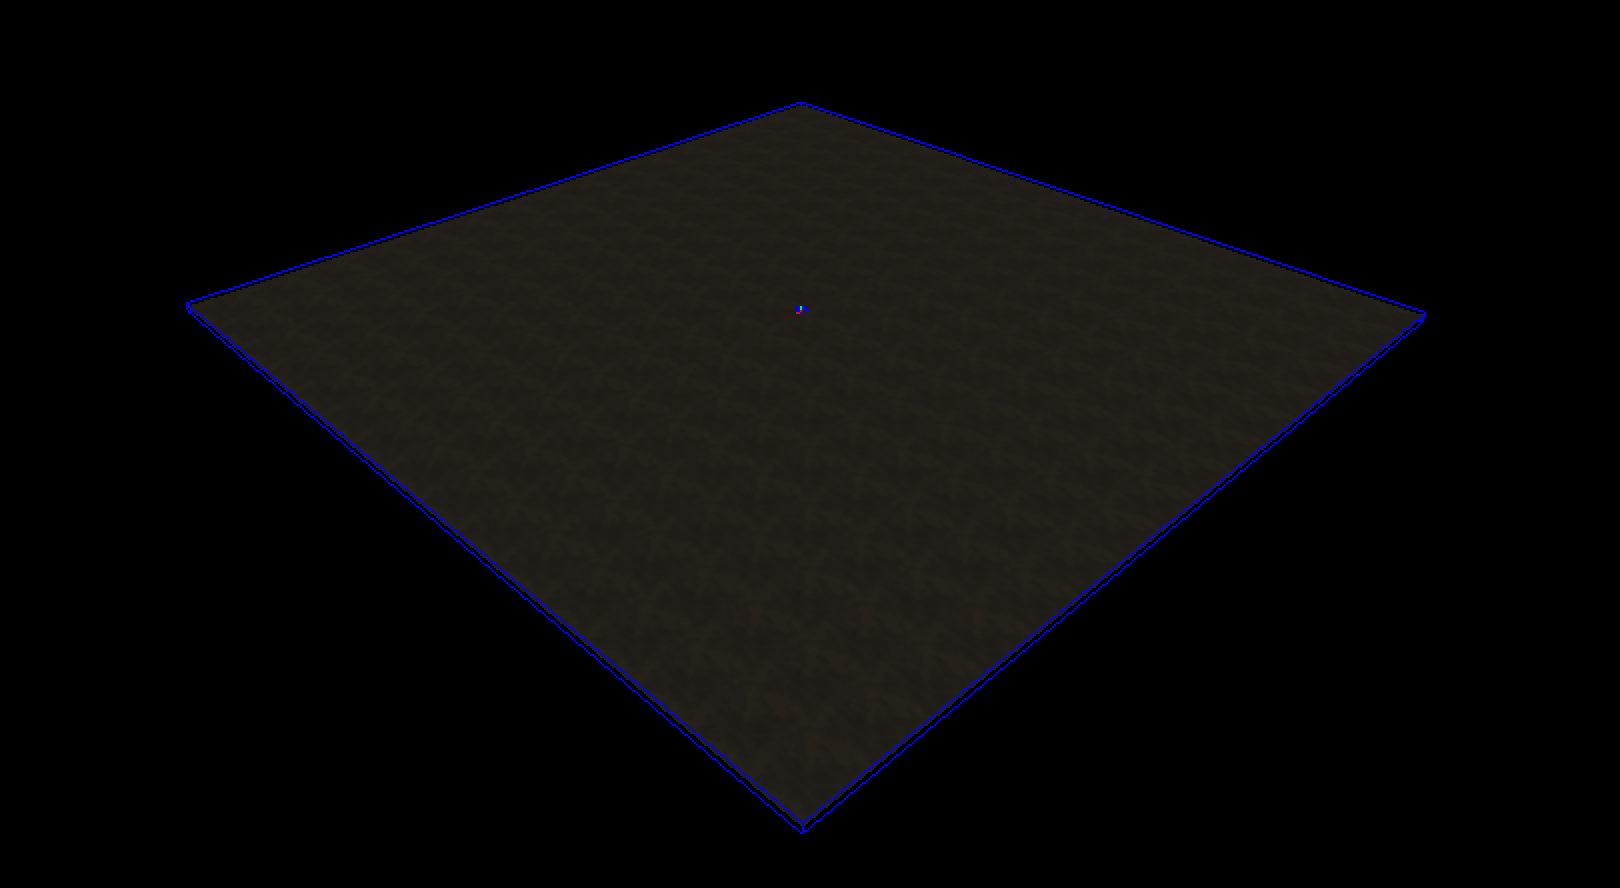
\includegraphics[width=.8\linewidth]{images/EmptySceneWithTerrain} 
	
\end{figure}
Nun kann man der Spielumgebung noch einige Modelle hinzufügen, sodass eine Welt entsteht, in der man sich während des Spiels bewegen kann. Modelle bekommt man relativ schnell und einfach über das Internet, wobei diese meistens nicht für die jMonkeyEngine konstruiert sind, sodass man diese noch konvertieren muss. Man kann diese 3D-Modelle in einem 3D-Tool importieren und für die jMonkeyEngine exportieren. Dies ist jedoch leichter gesagt als getan, denn viele Modelle verwenden Features, die nicht mit der jMonkeyEngine kompatibel sind. So benutzen viele Designer statt einer Lamp eine Sun als Lichtquelle, oder Modifiers, welche das Modell leicht verändern. Es war nicht immer einfach gute Modelle zu finden, die man in der jMonkeyEngine ohne viel Aufwand benutzen kann. Um ein eigenes Spiel wirklich komplett zu programmieren empfiehlt es sich, sich mit dem Design von 3D-Modellen auseinander zu setzen, wodurch man diese Mechanismen des Imports besser verstehen kann. Auf dieser Basis kann man zusätzlich sich eigene Modelle erstellen, welche wirklich zu dem eigenen Spiel passen. 

Möchte man der Welt neben ein paar Modellen außerdem eine realistische Umgebung geben, so darf man den Himmel nicht vergessen. Auch hier hat die jMonkeyEngine vorgefertigte Libraries und in der 
Terrain oder SceneComposer, sky,  
Funktionalität und allgemeines vorgehen.
Wichtig: Beschreibung von Licht nicht vergessen (sonst dunkel)

\subsection{Hinzufügen von Audio}
Bei großen rollen-basierten Spielen erzeugen die Sound-Effekte, neben den grafischen Eigenschaften, den Hauptbestandteil der entsprechenden Atmosphäre. In unserem Spiel wurden folgende Sound-Effekte verwendet:
\begin{enumerate}
	\item Horror-Theme Soundtrack als Hintergrundmusik
	\item Donner-und Regensounds, welche zufällig abgespielt werden
	\item Fußstapfen im Wald
	\item Spezial Effekte wie beispielsweise: Knisterndes Feuer, Wolfs-Heulen, Spieler-Atmen, Herzklopfen...
\end{enumerate} Um Audio dem Spiel hinzuzufügen sind beispielhaft die folgenden Code-Zeilen notwendig (bei bereits existierender Instanz-Variable).

\begin{lstlisting}
audio_nature = new AudioNode(assetManager,"Sound/nature.mp3", true); // Laden
audio_nature.setLooping(true);  // Aktiviere wiederholendes Abspielen
audio_nature.setPositional(true); // Raeumliche Audio-Effekte  
audio_nature.setVolume(3); // Lautstaerke festlegen
rootNode.attachChild(audio_nature); 
audio_nature.play(); // Abspielen des Sounds
\end{lstlisting}


\subsection{Physikalische Modellierung}
Die jme3 Engine erlaubt durch ihre Physik-Engine Objekten verschiedenes physikalisches Verhalten zuzuordnen. Die Kräfte, welche wirken sind dann je nach Masse verschieden.\\
In unserem Spiel haben wir hauptsächlich von der Schwerkraft Gebrauch gemacht, welche sich durch den Befehl\emph{ setGravity()} auf Spatials anwenden lässt.

\subsection{Effekte und Details}
Um dem Spiel mehr Leben einzuhauchen können verschiedenste Spezialeffekte erstellt werden. Im Folgenden wird auf zwei wichtige Beispiele eingegangen und wie diese in der jMonkeyEngine umgesetzt werden können.
\subsubsection{Nebel}
In unserem Wald haben wir zur besseren Atmosphäre einen Nebeleffekt hinzugefügt. Genaugenommen ist dies lediglich eine Erhellung der Pixel in Abhängigkeit des Abstandes vom Spieler. Es gibt zwei Möglichkeiten im Code Nebel zu erzeugen:
\begin{enumerate}
	\item[1.] Programieren eines Shaders 
	\item[2.] Verwendung des FogFilters in jme3
\end{enumerate}
Da wir uns für die Theorie dahinter interessierten haben wir uns über das allgemeine Vorgehen für 1. informiert aber letztendlich den FogFilter verwendet.
Die Berechnung des Nebels erfolgt exponentiell mit Berücksichtigung von Lichteffekten, abhängig vom Abstand zum Spieler. Entsprechende Erklärungen können unter \cite{Cr14} nachgeschlagen werden.

\begin{equation}
	FinalFogColor = (1.0-e^{db\textrm{1}})*fogColor + e^{db\textrm{2}} * lightColor \\
\end{equation} Wobei \\ \emph{
	d = Abstand zum Spieler} \\
	\emph{b = Nebeldichte je nach Lichteffekt} sind.


\begin{figure}[h!]
	\myfloatalign
	\caption{Exponentieller Nebel - Ergebnis}
	
	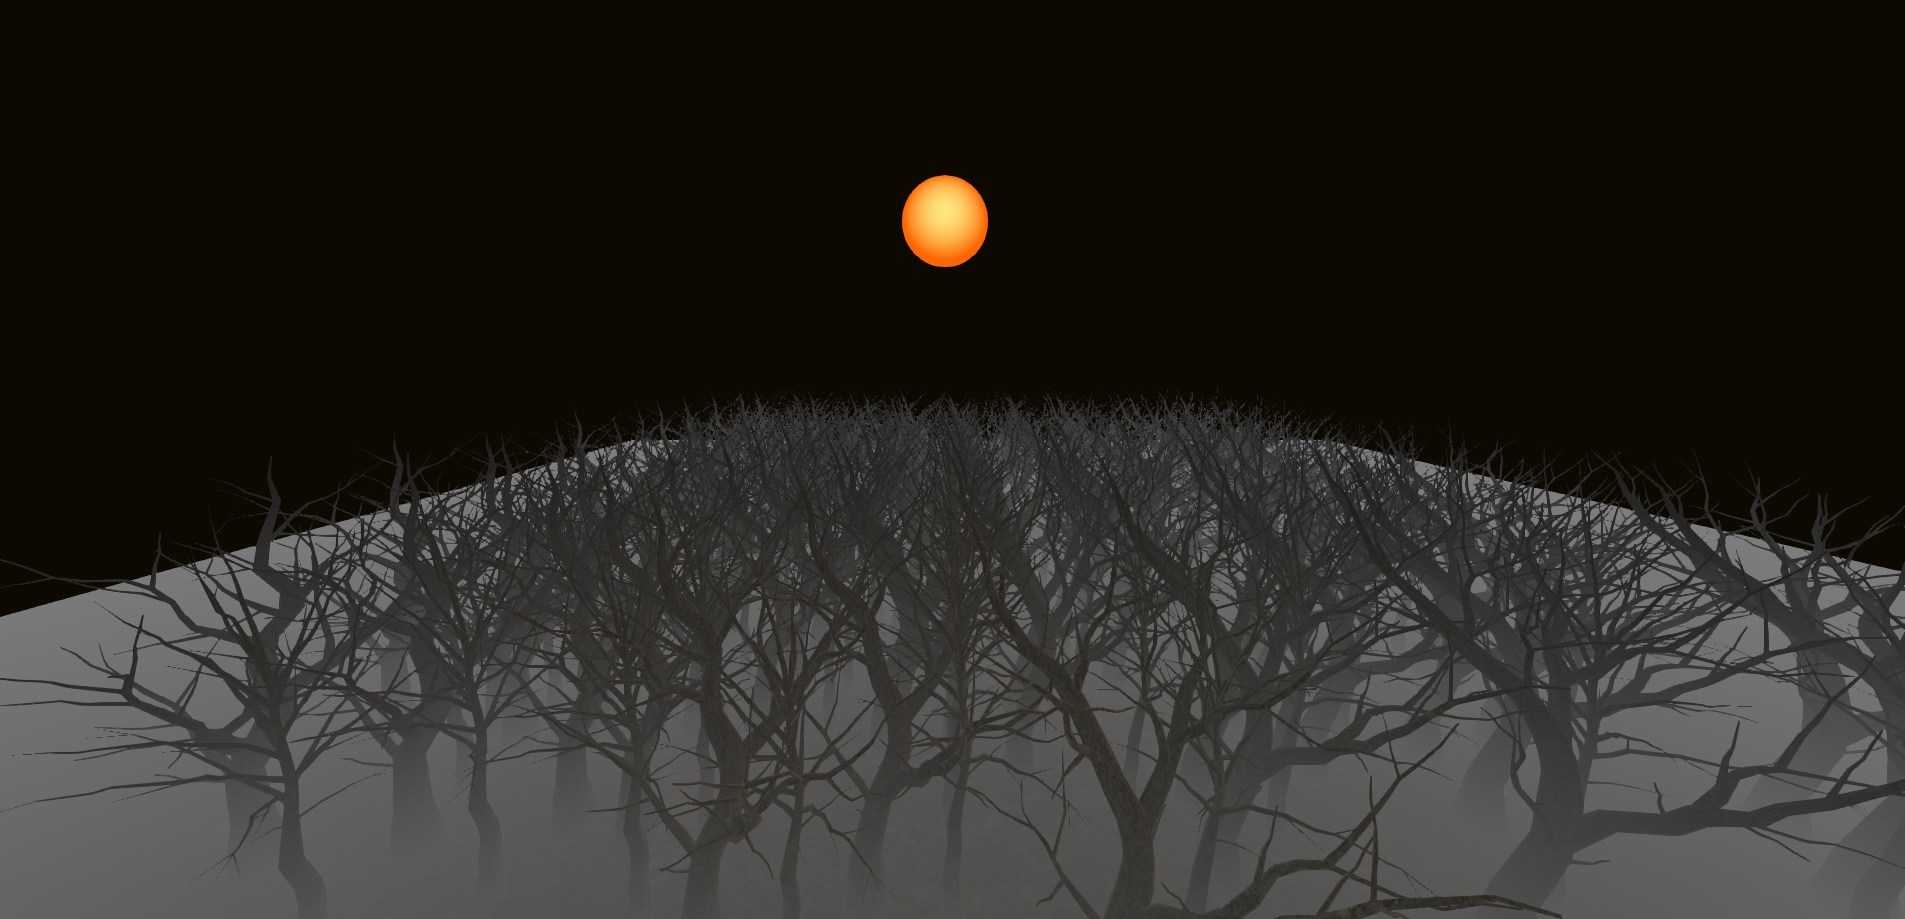
\includegraphics[width=.9\linewidth, height = 200pt]{images/fog} 
	
\end{figure}

\subsubsection{Partikeleffekte}
In fast jeder 3D-Game-Engine existieren Partikeleffekte. Dabei werden Partikel verschiedenster Formen und Größen mit unterschiedlichen Geschwindigkeiten in den Raum gezeichnet. Dadurch lassen sich beispielsweise Effekte wie ein brennendes Feuer, Schnee, Regen oder Explosionen erstellen. In jme3 existiert hierfür die Klasse \emph{ParticleEmitter}, welche sich um das Verhalten der Partikel kümmert.\\
In unserem Progman-Spiel kam diese in zwei Fällen zur Anwendung: Leichter Regen, sowie ein kleines Feuerchen in der nähe eines Hauses.\\ Im Folgenden ein Code-Beispiel wie Partikeleffekte erzeugt werden können, sowie Ausschnitte aus unserem Spiel.

\begin{lstlisting}
ParticleEmitter pm = new ParticleEmitter("effect", Type.Triangle, 60);
Material pmMat = new Material(assetManager, "Common/MatDefs/Misc/Particle.j3md");
pmMat.setTexture("Texture", assetManager.loadTexture("Effects/rain.png"));
pm.setMaterial(pmMat);
pm.setImagesX(1);
pm.setImagesY(1);
rootNode.attachChild(pm);
\end{lstlisting}


\section{Optimierung des Programms}\label{sec:optimizing}
Wenn man wie oben beschrieben einige Modelle und Effekte in seine Spielumgebung einbindet, können der Prozessor bzw. die Grafikkarte sehr schnell an Grenzen stoßen. Dabei spielt die Anzahl der Vertexes bzw. Triangles eine zentrale Rolle. Jedes Modell hat unter Umständen einige tausend Triangles, sodass sich dies in einem Spiel sehr leicht aufsummieren kann. In unserem Spiel gibt es zum Beispiel knapp 2000 Bäume, welche alle gerendert werden müssen: Vereinfacht man dort das Modell des Baumes, hat dies viel Potenzial, das gesamte Spiel zu beschleunigen. Mit Hilfe von \emph{F5} kann man in jMonkey während des Spiels anzeigen lassen, wie viele Triangles und Vertexes gerade zu rendern sind. Es versteht sich von selbst, dass ein Spiel mit einigen Millionen Vertexes viel zu aufwendig wird, weshalb die Framerate meist auf nahezu null sinkt. Um dies zu verhindern, muss man also die Anzahl an Triangles und Vertexes verringern. Dies ist grundsätzlich durch die Minimierung der Anzahl von Modellen oder durch die Minimierung der Anzahl an Triangles und Vertexes innerhalb eines Modells möglich. Diese haben dafür oft ein sogenanntes LevelOfDetail (kurz LOD), welches je nach Level ein Modell genauer zeichnet. Hier könnte man implementieren, dass das Modell genauer gezeichnet wird, wenn die Distanz zu dem Modell klein ist.

Interessanterweise fiel uns auf, dass das Terrain selbst (also der Untergrund des Spielers) sehr viele Triangles besitzt. Das liegt daran, dass das Terrain dafür ausgelegt ist, aufwendige Umgebungen darzustellen (sog. \emph{heightmaps}). So können Gebirge oder sonstige Unebenheiten sehr fein erstellt werden. Der Nachteil dabei ist jedoch, dass es sehr aufwendig wird das Terrain selbst ohne Models zu rendern, obwohl diese wie in unserem Beispiel einfach nur gerade sein kann. Es ist also unbedingt notwendig bei der Programmierung eines 3D-Spiels auf die Framerate und Komplexität der Welt zu achten.



\subsubsection{Minimierung der Anzahl von Modellen}
Um eine hohe Spielgeschwindigkeit zu gewährleisten bietet sich vorerst an, das Spiel möglichst simpel zu halten. Dies kann zum Beispiel erreicht werden, indem die Anzahl der benutzten Modelle reduziert wird. Also sollte man keine unnötigen Modelle verwenden, die nicht gebraucht werden. Man könnte zum Beispiel Modelle, welche von der Kameraposition im Spiel weit entfernt sind ausblenden, da diese sowieso nicht gesehen werden. In jMonkey kann man die Distanz einstellen, ab welcher die Modelle nicht mehr gerendert werden. Hier ein Beispiel aus unserem Code


\begin{lstlisting}
camera.setFrustumPerspective(45f, (float)cam.getWidth() / cam.getHeight(),1f,400f); //nur bis 100 Meter
\end{lstlisting}


Somit muss in unserem Beispiel nicht jeder der fast 2000 Bäume gerendert werden, sondern nur in der Nähe des Spielers. Auf diesem Weg kann sehr einfach die Komplexität der darzustellenden Welt reduziert werden.

\subsubsection{Level of Detail (LOD)}
In der jMonkeyEngine ist es grundsätzlich vorgesehen, dass man seinen Modellen eigene LODs gibt. Damit kann man anhand dieser LODs die Komplexität des Models im Laufe des Spiels bzw. vor dem Spiel verändern, indem man das Level of Detail ändert. Dabei gilt es noch zu beachten, dass die Modelle selbst keine LODs haben, sondern die Geometries, welchen sie zugrunde liegen. Man kann innerhalb des SceneExplorers die einzelnen Geometries in den Modellen auswählen, und so eigene LODs generieren:

\begin{center}
	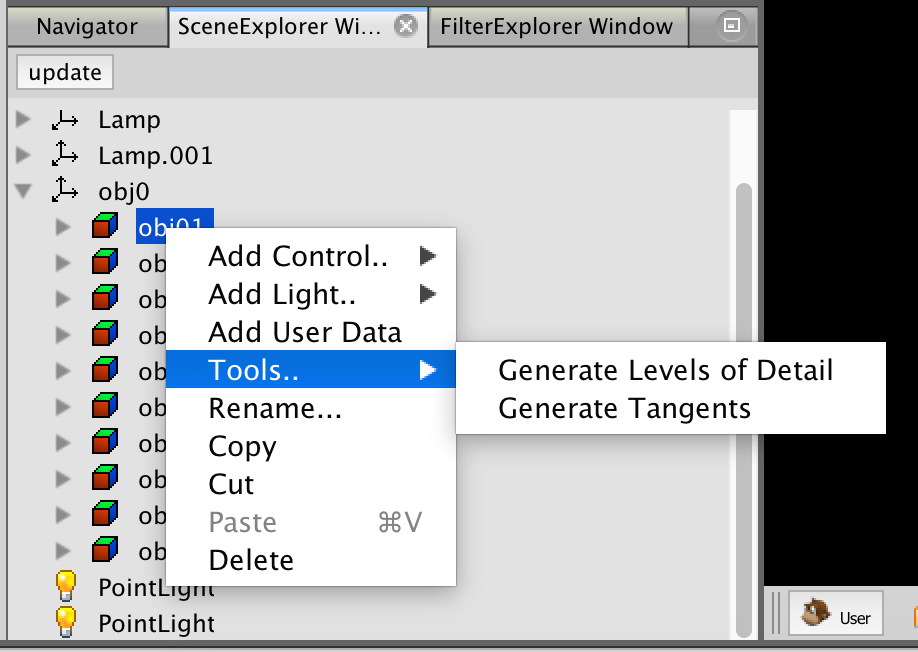
\includegraphics[width=0.7\linewidth]{images/generateLOD.png}
\end{center}

Ein alternativer Weg ist, dass man der Geometry eines vorhandenen Spatials während der Laufzeit über den Java-Code neue LODs zuweist. Dies hat den Vorteil, dass man die LODs dynamisch während der Laufzeit neu erstellen kann. Ein anderer Grund kann sein, dass man das Modell, das man benutzen will, nicht bearbeiten kann. Bei den Bäumen die wir in unseren Spiel benutzt haben kann man zum Beispiel über den SceneComposer keine LODs hinzufügen, da das Modell des Baums nur in der Testdata Library von jMonkey enthalten ist. 
Als Erstes muss für jede Geometry ein LodGenerator erstellt werden. Danach muss die bakeLods Methode aufgerufen werden, welcher man die ReductionMethod und den reductionValue übergeben muss. Es gibt drei verschiedene Methoden: Die am häufigsten benutzte Methode ist die PROPORTIONAL Methode, welche die Polygone um einen gewissen Prozentsatz reduziert. Die COLLAPSE\_COST Methode reduziert die Anzahl der Ecken solange, bis die Reduktionskosten den übergebenen Wert erreichen. Die CONSTANT Methode entfernt die gegebene Anzahl an Polygonen.
\begin{lstlisting}
LodGenerator lod = new LodGenerator(geometry);
lod.bakeLods(reductionMethod,reductionValue);
\end{lstlisting}

Der Methode bakeLods kann man auch mehr als nur ein reductionValue übergeben und somit mehrere LODs erstellen. Die LODs sind so gedacht, dass sie das Spiel vereinfachen, nicht, dass die Welt verunstaltet wird. Ein stark vereinfachtes Modell kann dem Spieler leicht negativ auffallen. Deshalb ist es sinnvoll, das Level of Detail während des Spiels automatisch anzupassen. Dafür gibt es die vorgefertigte LodControl Klasse, welche sicherstellt, dass das Level of Detail ausgehend von der Distanz zwischen Kamera und dem Modell gesetzt wird, hier ein Beispiel:

\begin{lstlisting}
LodControl lc = new LodControl();
lc.setTrisPerPixel(trisPerPixel);
myPrettyGeo.addControl(lc);
rootNode.attachChild(myPrettyGeo);
\end{lstlisting}


\section{Kritik an der jMonkeyEngine3}
Wir haben die jMonkeyEngine ausgewählt, weil sie komplett Java basiert ist, und weil sie eine gute SDK hat, in der man sehr einfach und schnell sein erstes 3D Spiel erstellen kann. Die Funktionen, die die jMonkeyEngine hat sind vielfältig. Wir möchten in diesem Abschnitt nun darauf eingehen, was wir für Erfahrungen mit der jMonkeyEngine gemacht haben. Die Grundlagen eines Spiels zu legen fiel uns leicht, denn dazu konnte man die Tutorials gut zu Rate ziehen, jedoch sind wir mit der Programmierung mit der jMonkeyEngine schnell an Grenzen unseres Wissens gestoßen, und haben auch im Internet wenig hilfreiches gefunden. Glaubt man jmonkeyengine.org, hat die jMonkeyEngine eine sehr gute Community und viele Probleme sind bereits geklärt worden. Doch als wir beim Programmieren einige Probleme hatten, war eben dies nicht gegeben. Man findet zwar oft einen entsprechenden Foreneintrag, der jedoch das Thema nicht genau trifft. Liest man den Eintrag nun durch, versteht man als Anfänger wenig, da sich dort häufig Experten unterhalten. Dazu komm, dass sehr viele Foreneinträge bereits einige Jahre alt sind und damit auch deren Links und Verweise auf andere Foreneinträge nicht mehr existieren. Man hat den Eindruck, als sei die Community vor einigen Jahren aktiv gewesen, jedoch nicht mehr heute. Sucht man bei Google das Wort "jMonkey", so findet man 113.000 Ergebnisse, sucht man stattdessen andere Engines wie "unity engine", so findet man 15.100.000, oder "cry engine" 11.600.000. Neben der nicht überzeugenden Dokumentation gibt es viele Fehler innerhalb von jMonkey oder der SDK. Das Erstellen eigener LODs hat zum Beispiel nur bei einem von uns beiden funktioniert, bei dem anderen ist einfach nichts passiert. Oder beim Arbeiten mit einer großen Scene Datei konnte der SceneComposer die Datei plötzich nicht mehr öffnen. Außerdem gibt es Fehler in den jMonkeyLibraries: In der SpotLight Klasse aus dem Paket com.jme3.light gibt es ein unnötiges System.out.println. Dort wird im Konstruktoraufruf ein berechneter Winkel in der Konsole ausgegeben. Sucht man dieses Problem, so stößt man darauf, dass das wohl jemand vergessen hat zu entfernen und den Bug nun beseitigt hat. Doch die letzte stabile Version hat dieses Problem immernoch. Beim benutzen eigener (bzw. online öffentlich verfügbarer) Modelle kann es sehr schnell zu Problemen führen, die auch oft nicht weiter spezifiziert werden. Beim transformieren und exportieren von 3D Modellen in jMonkey gab es oft Probleme, die nicht leicht zu beheben waren. Selbst die enge Zusammenarbeit mit Blender hat nicht wirklich gut funktioniert.
Zusammengefasst kann man sagen, dass die jMonkeyEngine eine sehr gute Engine ist, die viele Funktionen beinhaltet und dazu sehr variabel anpassbar ist, jedoch auch ihre Schwächen und längst nicht die riesige Community hat, wie sie es angeben. Gerade als Anfänger in der Spieleprogrammierung kann dies schnell zum Stocken führen.

